\section{Ionized Gas}
A plasma is considered to be a form or subset of ionized gas. That is, a volume
of neutral atoms or molecules, of which some fraction has been separated into
electrons and ions. For a sufficiently large number of particles, the behavior
of each species in the ionized gas can be described by a continuous distribution
function which specifies the number of particles with a specific range of
velocities, in a specific volume, at a specific time. This function is denoted
$f_\alpha(\vec{r_\alpha}, \vec{v_\alpha}, t)$, where the subscript $\alpha$
denotes the species, $f$ is the probability distribution, $\vec{r}$ is the
position, $\vec{v}$ is the velocity, and $t$ is the time.

The behavior of $f_\alpha$ can be shown to be governed by the Boltzmann
equation,
\begin{equation}\label{eq:boltzmann}
  \frac{\partial f_\alpha}{\partial t} + \vec{v_\alpha}\cdot\nabla f_\alpha +
  q_\alpha \left(\vec{E} + \vec{v_\alpha}\times\vec{B}\right)
  \cdot \nabla_v f_\alpha = \left( \frac{\partial f_\alpha}
  {\partial t}\right)_\mathrm{coll}.
\end{equation}
Here, $q$ is the charge of the species, $\vec{E}$ is the electric field,
$\vec{B}$ is the magnetic field, and $\partial f_\alpha/(\partial
t)_\mathrm{coll}$ is a term which represents changes to the distribution
function as a result of collisions. Coupled with Maxwell's equations,
equation~\ref{eq:boltzmann} provides a complete description of the behavior of
the fields and particles in a plasma.

For a species in equilibrium in the absence of external forces, ($\partial
f_\alpha/\partial t)_\mathrm{coll} = 0$, it can be shown that the distribution
of energies is
\begin{equation}\label{eq:mb}
  f_{\alpha}(\epsilon) = \frac{3\sqrt{3}}{\sqrt{2\pi}}(\kB T_\alpha)^{-3/2}
                        \exp{\left(-\frac{3\epsilon}{2\kB T_\alpha}\right)}
\end{equation}
where $\epsilon$ is the energy, $\kB$ is Boltzmann's constant, and $T_\alpha$ is
the temperature of the species. This is referred to as the Maxwell-Boltzmann
distribution. It must be emphasized that this solution only applies to
situations where the species can be considered to be in equilibrium. Gradients
and electromagnetic fields can both drive a distribution far from this
equilibrium condition. This is particularly important when plasmas are discussed
in the context of temperature.

A solution to equation~\ref{eq:boltzmann} may also be derived in the case of a
relatively small electric field and only elastic collisions. This result was
originally presented by Druyvesteyn and Penning \cite{Druyvesteyn1940} and has
come to be known as the Druyvesteyn distribution. It is defined as,
\begin{equation}
  f_{\alpha} = \frac{3\sqrt{3}}{4\Gamma(3/4)}(\kB T_\alpha)^{-3/2}
  \exp{\left[-\frac{9}{16}\left(\frac{\epsilon}{\kB T_\alpha}\right)\right]}
  \label{eq:druy}
\end{equation}
where $\Gamma$ is the gamma function. This solution tends to suppress the
probability of higher and lower-energy electrons in favor of more intermediate
values. Figure~\ref{fig:simpledists}
\begin{figure}
  \centering
  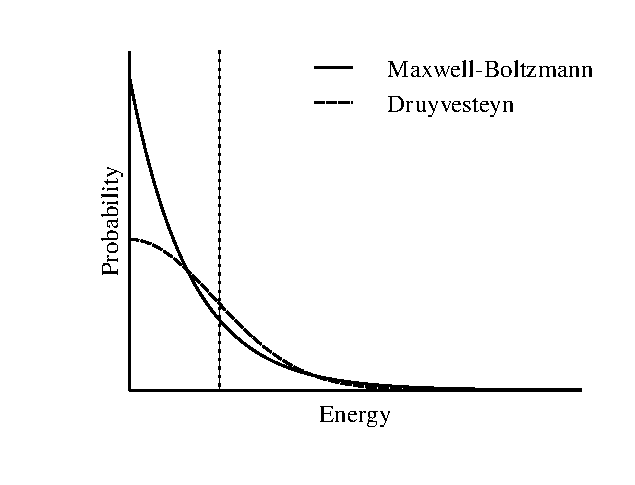
\includegraphics{./chapters/theory/figures/simpledists.eps}
  \caption{Comparison of the Maxwell-Boltzmann energy distribution and the
    Druyvesteyn distribution for the same average energy (illustrated by the
  dotted line).}
  \label{fig:simpledists}
\end{figure}
compares the probably distributions from equations~\ref{eq:mb}
and~\ref{eq:druy} for the same temperature $\T_\alpha$. The dotted line
illustrates the average energy for the two distributions, which is not the same
as the most probably energy.

Additional solutions of equation~\ref{eq:boltzmann} in anything but these simple
cases can be very challenging. It most situations, it is reduced to more tenable
equations by integrating over the velocity-space (leaving $f$ as only a function
of space and time). The first so-called moment is often called the conservation
equation or continuity equation,
\begin{equation}\label{eq:cont}
  \frac{\partial n_\alpha}{\partial t} + \nabla \cdot (n_\alpha \vec{u_\alpha})
  = G_\alpha - L_\alpha.
\end{equation}
In this case, $\vec{v}$ has been replaced by a mean velocity $\vec{u}$. We have
also introduced terms losses ($L$) and gains ($G$) in the species density.

The definition of the mean velocity can be obtained by multiplying
equation~\ref{eq:boltzmann} by $v$ and integrating over velocity-space. This is
referred to as the second moment. The result is an equation expressing the
conservation of momentum for the species. The actual equation will not be
reproduced here, but it forms the basis for the two-fluid approximation of a
plasma. In the course of developing the second moment an additional term, the
pressure tensor, is introduced which can only be defined by the third moment of
equation~\ref{eq:boltzmann}. In fact, each additional moment introduces a new
term, \emph{ad infinitum}. For most cases, the first two or three moments
suffice, after the sequence is terminated by the use of an additional
assumption.

For our purposes, one more moment will suffice. Multiplying by $mv^2/2$,
integrating over velocity-space, and assuming that the pressure is isotropic,
produces the energy conservation equation,
\begin{equation}
  \frac{\partial}{\partial t}\left(\frac{3}{2}p_\alpha\right) 
  + \nabla\cdot\frac{3}{2} (p_\alpha\vec{u}_\alpha)
  + p_\alpha\nabla\cdot\vec{u}_\alpha
  + \nabla\cdot\vec{q}_\alpha
  = \frac{\partial}{\partial
  t}\left(\frac{3}{2}p_\alpha\right)\bigg|_\mathrm{coll}.
\end{equation}
In this case, $p$ represents the plasma pressure, and $\vec{q}$ is the heat
flow. The first term on the \textsc{lhs} represents the total energy contained
by the species, the second term is the energy flux in and out of the volume, and
the third term accounts for changes due to compression or expansion. The
\textsc{rhs} is the collision operator which describes energy added or removed
from the system as a result of collisions.

\section{Plasma Criteria}
While equations above can equally describe an ionized gas or a plasma, the two
are conceptually distinct. A plasma is unique in that its dynamics are governed
by long range electromagnetic forces, unlike gases in which short-range
collisions dominate. As a result, plasmas frequently feature large scale
structure and organization. Examples of these structures are ubiquitous in
astronomy where phenomena such as the aurora borealis, coronal mass ejections,
and even interstellar media all qualify as forms of plasma. How then, does one
define a plasma? There are three criteria required of an ionized gas in order
for it to be considered a plasma.

\subsection{Debye Length}
An ionized gas is composed of both positive and negative charges, usually some
combination of ions and electrons. If an electrical perturbation is introduced,
the charge particles will tend to rearrange themselves to shield out the effect
of the perturbation. A plasma is an ionized gas which is sufficiently large for
this shielding effect to occur. The length scale of this shielding effect is
referred to as the Debye length, denoted $\lambda_D$. The Debye length can be
shown to be equal to $\sqrt{\epsilon_0T_e/(en_0)}$, where $\epsilon_0$ is the
vacuum permittivity, $T_e$ is the electron temperature, and $n_0$ is the plasma
density. If the characteristic length scale of the ionized gas is $L$, then
$\lambda_D < L$ for it to be considered a plasma.

\subsection{Debye Sphere}
However, the previous condition is necessary, but not sufficient for shielding
to occur. It is possible to have an ionized gas in which the Debye length is
smaller than the characteristic length scale, but in which there are too few
charged particles for shielding to occur. More simply put, it would be
impossible for a single electron to shield out even the smallest of
perturbations. For that reason, the number of particles in a Debye sphere must
be greater than unity in a plasma, or {$n_0(4\pi \lambda_D^3/3) >> 1$.

\subsection{Plasma Oscillations}
If an ionized gas meets the two aforementioned conditions, it may still not
exhibit the large scale structure of plasma if the collision frequency with
neutral particles is too high. In this case, the behavior of the ionized gas
would be determined more by the random collisions with gas particles than the
long-range electromagnetic forces. As a result, the characteristic oscillation
frequency of a plasma (or plasma frequency) $\omega_p$ must be greater than the
neutral collision frequency, $\nu$, or {$\omega_p > \nu$}. Here, $\omega_p =
\sqrt{e^2n_0/(\epsilon_0 m_e)}$.

In spite of this range of requirements, there are a large number of natural and
man-made plasmas. Figure~\ref{fig:regimes}
\begin{figure}
  \centering
  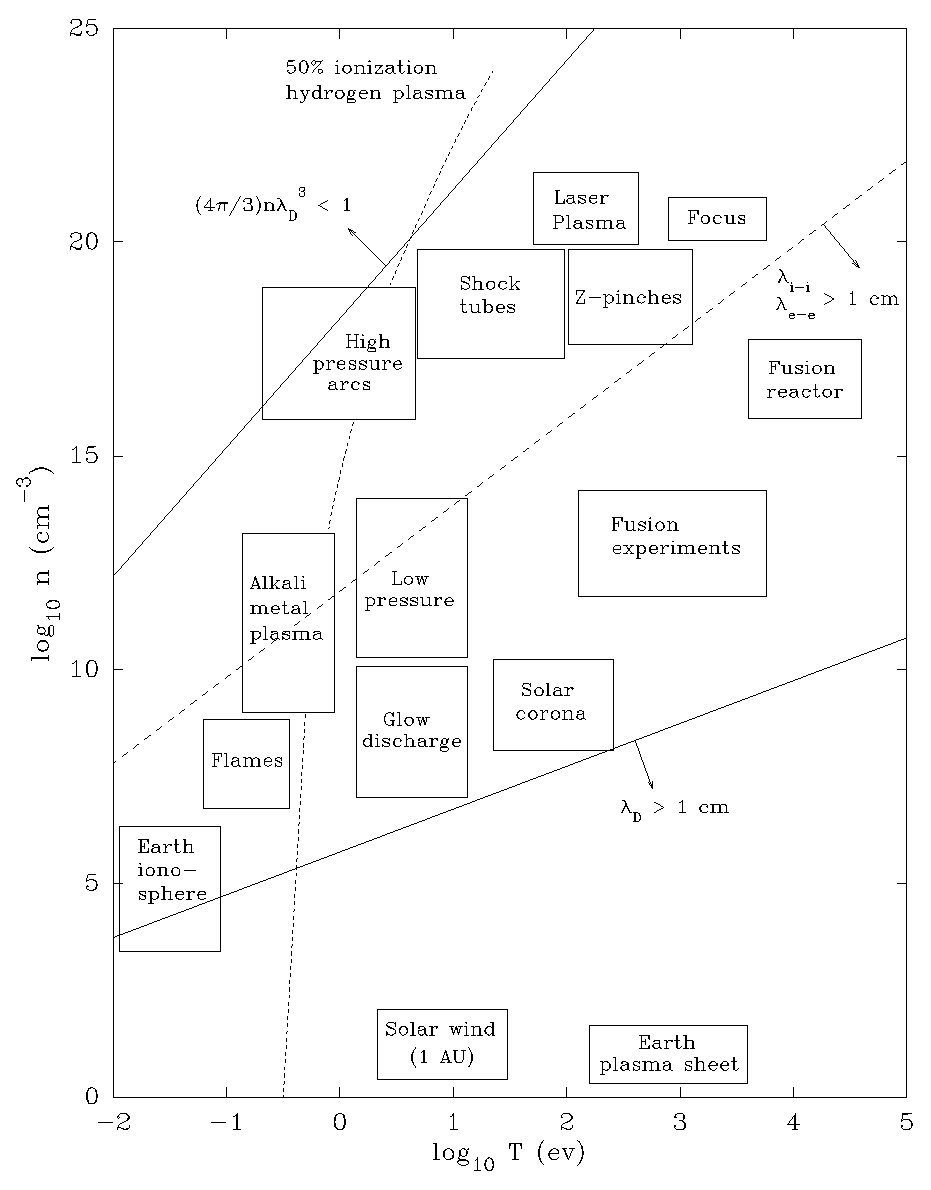
\includegraphics{./chapters/theory/figures/regimes.eps}
  \caption{Illustration of the various regimes of plasma in terms of
electron temperature and density \cite{Huba2011}.}
  \label{fig:regimes}
\end{figure}
shows several categories of plasma, plotted as a function of their electron
density and temperature. As can be seen, the electron densities span seven
decades, and the densities cover in excess of 20.

\section{Streamer Discharge}
The Boltzmann equation is a continuous, statistical description of a plasma. By
comparison, the initial breakdown of a plasma is a discontinuous process marked
by its stochasticity. The initiation of a discharge is the result of electron
avalanches which may occur randomly throughout the discharge, particularly
without any form of preionization. Often, the seed electrons for a plasma result
from ionizing cosmic rays which generate a few electrons per cubic-centimeter.

Classically, plasmas are created by two different mechanisms, depending on the
strength of the electric field. At lower electric fields, the Townsend mechanism
is used to explain the formation of a plasma. Consider a two electrodes
separated by a gap filled with some gas. An electron starting near the cathode
will drift toward the anode. For a sufficient electric field, the electron will
gain enough kinetic energy to ionize a neutral atom, creating two electrons.
These two electrons may then ionize additional neutral atoms as they cross the
gap, in a manner similar to that seen in fig~\ref{fig:avalanche}. Eventually,
the electrons are collected at the anode. However, in their wake are ions which
slowly drift toward the cathode. Upon colliding with the cathode, they have some
probability of emitting a secondary electron which will also undergo an
avalanche. Townsend breakdown occurs when the enough electron multiplication
occurs within the gap to balance out the ions which do not produce secondary
electrons.

This process is characterized by $\alpha$ and $\gamma$, the first and second
Townsend coefficients. $\alpha$ expresses the number of ionization events per
unit pathlength for a given electric field. On the other hand, $\gamma$ is the
probability that an ion impinging on the cathode produces a secondary electron.

In contrast, the streamer discharge does not rely on secondary emission
processes. Again, consider an electron between two electrodes, as seen in (a) of
figure~\ref{fig:streamer}.
\begin{figure}
  \centering
  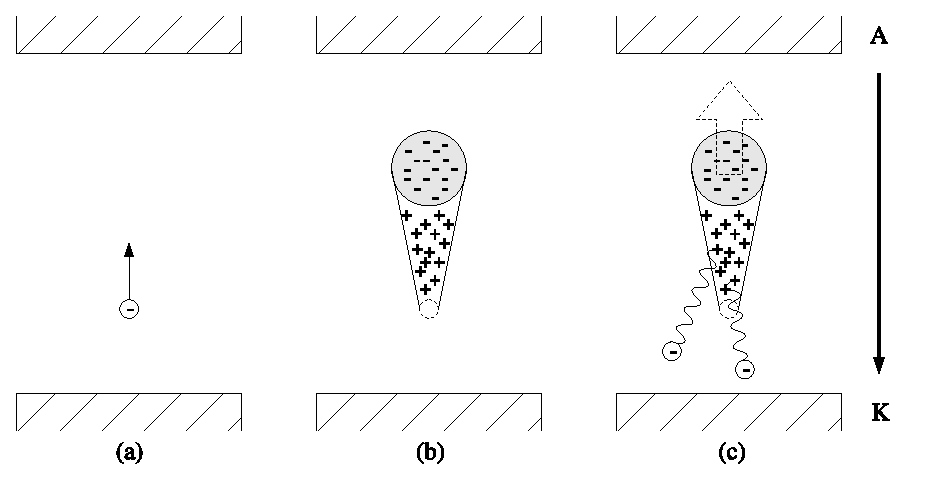
\includegraphics{./chapters/theory/figures/streamer.eps}
  \caption{An illustration of the development of a single streamer. (a)
    A seed electron is accelerated by the applied electric field. (b) The
    initial electron develops into an avalanche which leaves a large region
    of positive space charge, halting further advance. (c) The streamer
    propagates toward the cathode via photoionization and the anode via
    nonlocal electrons and photoionization.}
  \label{fig:streamer}
\end{figure}
The only difference from the Townsend case, is that the electric field is much
larger. Again, the electron acquires energy from the applied electric field, and
begins to create an avalanche of electrons. Following Levatter and Lin
\cite{Levatter1980}, the electrons in the avalanche travel with a velocity
characterized by the electron mobility, $\mu$. This term expresses the
frictional force exerted by the gas on the electrons. Consequently, the mean
velocity of electrons drifting in a field $E(t)$ can be expressed as
\begin{equation}
  u = \mu(E/N_g) E(t),
\end{equation}
where $N_g$ is the neutral gas density. This involves the implicit assumption
that the electrons in the avalanche have reached equilibrium with the applied
field at all times, $t$. Given this definition of the electron drift velocity,
the total length of the avalanche may be written as
\begin{equation}
  \xi = \int_{t_0}^t u dt.
  \label{eq:s_xi}
\end{equation}
Here, $t_0$ is the time at which $E(t)$ becomes sufficiently large for $\alpha >
0$ which is interpreted as the beginning of the avalanche.

As seen in figure~\ref{fig:streamer}, the ions generated by the ionization
events remain in place as the electron avalanche passes. This follows from the
much larger mass of the ions, and the relatively short time scale on which the
avalanche occurs (often on the order of nanoseconds). The cone-like structure of
the ions results from the collision-induced, transverse diffusion of the
electrons. The diffusion coefficient for can be approximated as $D = \lambda
v_mathrm{th}/3$, where $\lambda$ is the mean free path of the electrons, and
$v_\mathrm{th}$ is their thermal velocity. Assuming that the electrons diffuse
equally in the lateral transverse directions, the electron density in the head
of the avalanche is a sphere of the form,
\begin{equation}
  n_e(r) = \frac{N_e}{\pi^{3/2}R^2}\exp\left(-\frac{r^2}{R^2}\right),
  \label{eq:s_density}
\end{equation}
where $r$ is the radial coordinate (relative to the center of the avalanche),
$N_e$ is the electron population, $\Delta t$ is the time elapsed since $\alpha >
0$, and $R$ is the diffusion radius. The diffusion radius can be calculated from
\begin{equation}
  R = \int_{0}^{\xi} \lambda v_\mathrm{th}(\xi') d\xi',
  \label{eq:s_rad}
\end{equation}
as the thermal velocity is expected to change as more energy is deposited into
the electrons over the length of the avalanche.

In a Townsend discharge, the avalanche would be expected to cross the entire
width of the gap. For a streamer, on the other hand, the space charge of the
avalanche becomes sufficiently large that it stalls mid-gap as can be noted in
part (c) for figure~\ref{fig:streamer}. It is commonly assumed that this occurs
when the peak field within the head of the avalanche becomes equal to the
applied field. Again, from Levatter and Lin, electric field can be found to
equal,
\begin{eqnarray}
  E_a(r) = \frac{eN_e}{4\pi\epsilon_0R^2} F(r/R), \qquad \mathrm{where} \\
  F(r/R) = \frac{1}{R^2}\left[\mathrm{erf}(r/R)-\frac{2}{\pi^{1/2}}
           (r/R)\exp(-r^2/R^2)\right] ,
\end{eqnarray}
and $\mathrm{erf}$ is the error function. $F$ is a dimenionless function which
has a peak value of $0.428$. The number of electrons in the avalanche, is equal
to
\begin{equation}
  N_e = \int_0^\xi \alpha(\xi')d\xi'.
  \label{eq:s_pop}
\end{equation}

Levatter and Lin make a number of assumptions in order to develop an analytic
and dimensionless solution for $E_{a,\mathrm{max}}(t) = E(t)$. However, it is
possible to numerically integrate equations~\ref{eq:s_xi} and~\ref{eq:s_rad} so
as to more accurately calculate the final radius, and length of the avalanche.
Figure~\ref{fig:he_avalanche}
\begin{figure}
  \centering
  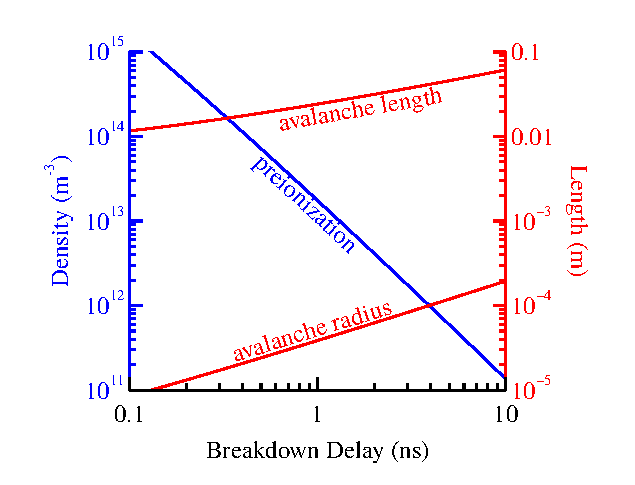
\includegraphics{./chapters/theory/figures/he_avalanche.eps}
  \caption{Numerical calculations of the preionization density for homogeneous
    excitation, avalanche length, and avalanche radius in helium at a pressure
    of 1.0 Torr as a function of the slope of the electric field.}
  \label{fig:he_avalanche}
\end{figure}
shows the results of such calculations for a streamer in 1.0 Torr of helium, and
various breakdown delays. The breakdown delay is the time it takes for $\alpha >
0$ with a linearly increasing electric field. The values for the mobility, mean
velocity, and Townsend coefficient were interpolated from solutions of the
Boltzmann equation provided by the \smaller{BOLSIG+} code with Phelps' cross
sections \cite{Phelps2002}. For this range of breakdown delays, the avalanche
length requires an anode-cathode gap of 1-6 cm for a streamer to form.

At this point the avalanche can no longer continue, and several processes are
responsible for the development of the streamer. For one, the large internal
field of the avalanche can ``inject'' electrons in the direction of the anode
\cite{Kunhardt1980}. In addition, excited atoms in the wake of the avalanche can
emit photons, ionizing the gas between the avalanche head and the anode. These
electrons are then subject to the large electric field between the anode and
avalanche head, resulting in additional avalanches. Likewise, photoionization
can occur in the region between the tail of the streamer and the cathode.
Together, these processes create a constricted conductive pathway which bridges
the two electrodes. The rapid flow of current through this conductive pathway
quickly thermalizes the plasma, eventually transitioning to an arc.

However, these later processes are not critical in the formation of a volume
discharge by an \acs{rpnd}. The original description of the streamer only treats
the result of a single avalanche. In reality, it is possible for several
avalanches to form simultaneously. Furthermore, with sufficient preionization,
the strong fields of the stalled avalanches can influence each other, smoothing
out the field gradients which constrict the streamer. This is roughly equivalent
to the case where the spherical avalanche heads overlap just at the stalling
condition. In that case, the condition for homogeneous breakdown is simply
$n_{e,c} > r_c^{-3}$, where $n_{e,c}$ is the preionization density, and $r_c$ is
the radius of the stalled avalanche. A plot of this condition with the breakdown
time can also be observed in figure~\ref{fig:he_avalanche}.

From this condition, it is apparent that as the avalanche radius increases, the
necessary preionization decreases. Less obvious is the increasing avalanche
radius with breakdown delay. The higher breakdown delay implies a slower slope
to the electric field and thus a longer time before the internal field of the
avalanche becomes significant. As a result, longer breakdown delays imply that
the avalanche has more time to diffuse, leading to the increased radius.

\section{Atomic Spectroscopy \& Notation}

Unlike physical probes, optical diagnostics are noninvasive and offer an
attractive approach to the measurement of plasma parameters. Careful
measurements of the light emitted from excited atomic states can yield electron
densities and temperatures, excited state densities and temperatures, electric
fields, and magnetic fields. The topic of spectroscopy is extensive and it is
neither necessary nor desirable to cover it in full. Instead we will only
consider what is necessary to understand the emissions from a singly-excited,
multi-electron atom.

An atom is composed of a small, positively charged nucleus, orbited by a
negatively charged electrons. The actual position of any single electron is
probabilistic and described by a wavefunction, as determined by solutions of the
Schr\"{o}dinger equation. Multiple possible wavefunctions or orbitals exist, and
the Pauli exclusion principle prevents more than one electron from possessing
the same orbital. Each orbital is identified by four quantum numbers,
\begin{itemize}
  \item $n=1,2,\ldots$: the principal quantum number,
  \item $l=0,1,\ldots,n-1$: the orbital angular momentum, and
  \item $s=\pm1/2$: the spin angular momentum.
\end{itemize}
The principal quantum number identifies the shell to which an electron belongs.
Each shell can contain a total of $2(2l+1)$ electrons, after which it is
considered full. Each shell has a series of subshells, defined by $l$ (using the
nomenclature $0,1,2,3,\ldots = s,p,d,f,\ldots$). 

The electrons of an atom possess potential energy as a result of their
separation from the nucleus. As $n$ and $l$ increase, so does the potential
energy, thus an electron in the 1s ($n=1$ and $l=0$) subshell has the lowest
possible potential energy. Each as a result of the exclusion principle, each
subshell can only contain up to $2(2l+1)$ electrons after which it is considered
full.

Absent from external influences, the subshells are populated with electrons so
as to minimize the potential energy of the system. This natural arrangement is
referred to as the ground state configuration. Often, but not always, the
subshells are filled sequentially and in order from lowest to highest $l$.
Provided some input energy, one or more of the electrons surrounding the atom
may transition to another orbital, increasing the potential energy of the
system. In low-temperature plasmas it usually one of the electrons from the
outermost or unfilled subshell to be excited.

In hydrogen-like atoms with a single electron in a single unfilled subshell, the
potential energy of any singly-excited configuration is uniquely determined by
this single outer electron. As a result, the initial and final states of the
atom can be uniquely identified based on the initial and final $n$ and $l$ of
aforementioned electron. In contrast, the potential energies of configurations
in noble gases and atoms with more than one electron in the valence shell are
determined by the collective effects of these outer electrons.

This necessitates an additional means of classifying the configuration of the
outer electrons. It turns out that the state of these types of atoms can be
specified based on their total orbital angular momentum $\bm{L}=\sum \bm{l}_i$,
the total spin, $\bm{S}=\sum \bm{s}_i$, and the total angular momentum,
$\bm{J}=\bm{L}+\bm{S}$, where $i$ are all the electrons of the unfilled shell.
In addition, each state can be said to have either even or odd parity, defined
as $(-1)^{\sum\bm{l}_i}$.

Together, these values can be used to express the term symbol for any particular
atomic state. For example, the so called triplet metastable state of helium can
be written as 1s2p$^3$P$^o_{0,1,2}$. This describes a helium atom with one
electron in the 1s subshell and a second atom in the 2p subshell. This
configuration has a total orbital angular moment of 1, odd parity (denoted by
the superscript `o'), a total spin of $1/2$ (the superscript $3$ is equal to
$2S+1$) and three possible values for the total angular momentum: 0, 1, or 2
which varies depending on the spin-orbit interaction.

These excited atomic states usually have finite lifetimes as the electrons in
the excited states will often transition to lower states. This can occur
spontaneously, through the emission of a photon, or via a superelastic collision
with another particle. In the case of spontaneous transitions, only certain ones
are allowed, as defined by a set of selection rules:
\begin{itemize}
  \item $\Delta S = 0$
  \item $\Delta L = \pm1$ or 0
  \item $\Delta J = \pm1$ or 0
  \item $L=0$ cannot transition to $L=0$
  \item $j=0$ cannot transition to $J=0$
\end{itemize}
These rules are determined using the electric dipole approximation. As a result,
some transitions forbidden by these rules can occur, though they occur with much
lower frequency.

Figure~\ref{fig:grotrian}
\begin{figure}
  \centering
  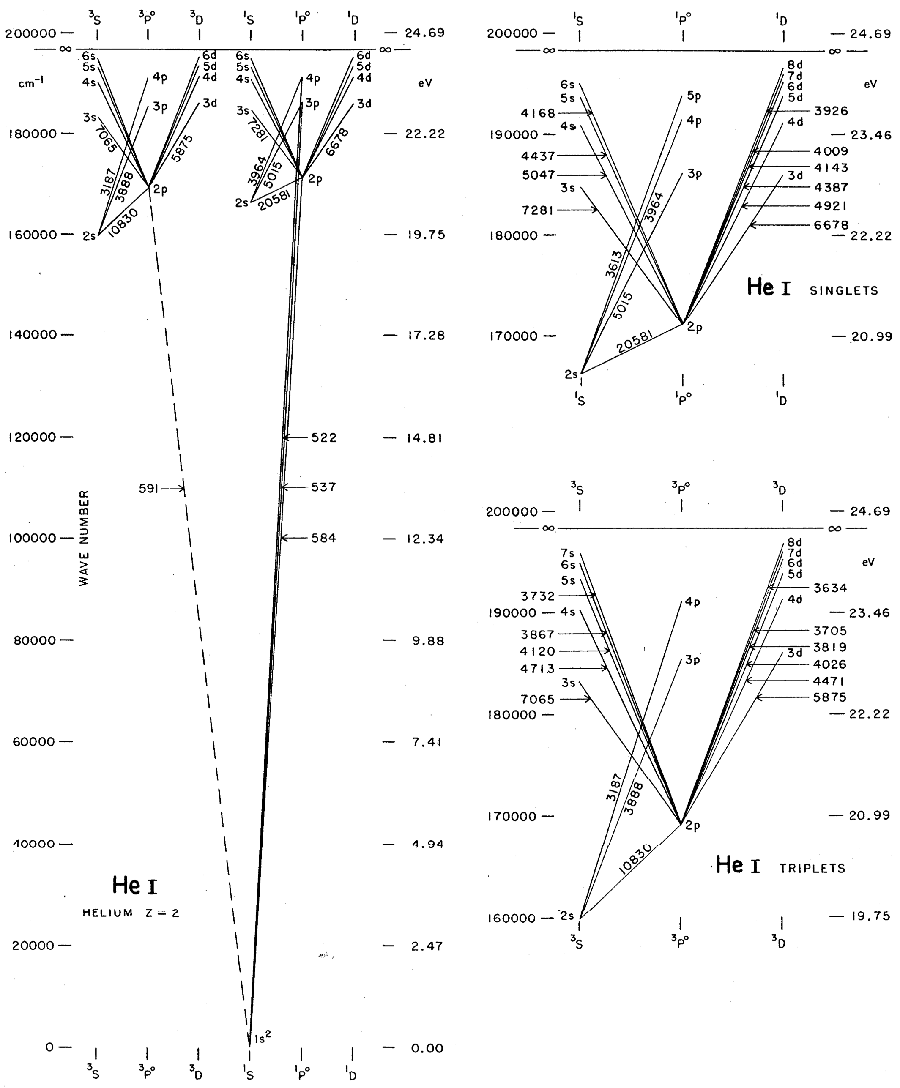
\includegraphics{./chapters/theory/figures/grotrian.pdf}
  \caption{A partial Grotrian diagram of neutral helium \cite{Moore1968}.}
  \label{fig:grotrian}
\end{figure}
is a diagram of the energy levels in neutral helium and the allowed transitions.
In this case, the atomic states are separated into the singlet and triplet
manifolds. The singlet manifold represents excited states where the electron
spins are anti-parallel, and the triplet manifold represents excited states
where the electron spins are parallel. As indicated by the first selection rule,
transitions between these two manifolds is forbidden, thus each is something of
a self-contained system.

\subsection{Spectral Lineshapes}

It is the transitions between these various excited states which concern
spectroscopy. Electrons which transition to lower energy states emit photons
which can be detected. Conversely, if an atom is subject to a photon with an
energy matching a transition, the photon may be absorbed. Both processes are
useful in determining the prevalence and dynamics of the excited states. This,
in turn, can be used to infer various plasma properties.

Conservation of energy requires that the energy of the absorbed or emitted
photon match the energy difference between the two states. However, the finite
lifetime of excited atomic states implies, via the time-energy formulation of
the uncertainty principle, some uncertainty in the actual energy difference
between the states. As a result, the emitted photon will possess an energy
selected from a distribution of energies.

This distribution is referred to as the spectral lineshape. The natural
lineshape of an atomic transition can be shown \cite{Siegman1986} to be a
Lorentzian of the form,
\begin{equation}
  g(\omega) = -\frac{1}{4\pi^2}\frac{A\lambda^3}{\dwa}
  \frac{1}{1 + \left[2(\omega-\omega_a)/\dwa\right]^2},
  \label{eq:lorentzian}
\end{equation}
where $\omega$ is the photon frequency, $A$ is the Einstein coefficient for the
transition, $\lambda$ is the wavelength of the transition, $\omega_a$ is central
frequency of the transition, and $\Delta\omega_a$ the full-width half maximum
(\acs{fwhm}) of the transition. In the ideal case, where the atoms motionless
and unaffected by external perturbations, $\Delta\omega_a = A$. This is known as
the natural linewidth.

Other processes can affect the spectral lineshape. For example, inter-atomic
collisions can reduce the lifetimes of excited states. This results in
additional broadening of the line, though it retains its Loretnzian nature. As
the frequency of inter-atomic collisions increases linearly with pressure, this
phenomena is referred to as pressure broadening. It can be included in
equation~\ref{eq:lorentzian} by using $\Delta\omega_a = A + BP$, where $B$ is a
measured or calculated broadening coefficient, and $P$ is the pressure.

Atomic motion can also play a role in the spectral lineshape. If an atom is
moving toward or away an observer as it emits a photon, the emitted photon will
be blue or red shifted. If this effect is averaged over the random motion of
atoms in a gas, the result is an additional broadening of the lineshape, called
Doppler broadening. Unlike pressure broadening, Doppler broadening introduces a
Gaussian component to the lineshape such that,
\begin{multline}
  g(\omega) = \sqrt{\frac{2\ln{2}}{\pi^3}}\frac{\dwa}{\dwd}
  \int_{-\infty}^\infty
  \frac{1}{[(\omega - \omega_a) - \omega']^2 + 4\dwa^2} \\
  \times \exp\left[4\ln{2}\left(\frac{\omega'}{\dwd}\right)^2\right]d\omega'.
  \label{eq:voigt}
\end{multline}
Here, $\dwd = \omega_a\sqrt{\frac{8k_\mathrm{B}T_\mathrm{g}\ln{2}} {Mc^2}}$, is
the width of the Doppler broadening. This form of the spectral lineshape is
known as the Voigt profile, and it must be numerically integrated. In the case
that $\dwd >> \dwa$, equation~\ref{eq:voigt} can be simplified to a standard
Gaussian distribution,
\begin{equation}
  g(\omega) = \sqrt{\frac{4\log{2}}{\pi\dwd^2}}
  \exp\left[-(4\log{2})\left(\frac{\omega-\omega_a}}{\dwd}\right)^2\right].
\end{equation}

The effect of the various broadening mechanisms is most apparent in the wings of
the lineshape, far from the peak. Figure~\ref{fig:lineshapes}
\begin{figure}
  \centering
  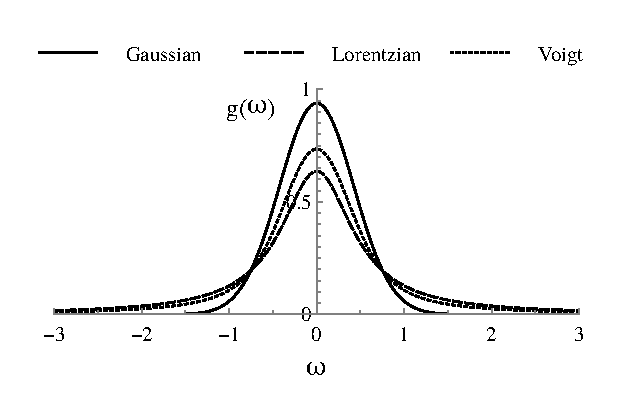
\includegraphics{./chapters/theory/figures/lineshapes.eps}
  \caption{A comparison of the three primary spectral lineshapes, each with the
  same full width.}
  \label{fig:lineshapes}
\end{figure}
illustrates the three major lineshapes with equivalent full widths. The Voigt
profile is composed of equally broad Lorentzian and Gaussian distributions. As
can be seen, the wings of the Gaussian distribution fall off very quickly. In
comparison, the Lorentzian component is observable well out to the edges of the
figure. 

The spectral lineshape can be altered by a number of other processes. Electric
fields can influence the emissions via the Stark effect, while magnetic fields
can split up degenerate states via the Zeeman effect. The fields of electrons
and nearby molecules can also alter the lineshape of a transition. While not
used in this study, such effects can be used as effective diagnostic tools for
plasmas.
